\documentclass{beamer}
\usepackage[utf8]{inputenc}
%\usepackage[brazil]{babel}
\usepackage{tcolorbox}
\usepackage{lipsum}
\usepackage{framed,color,verbatim,tikz,wrapfig,ragged2e,textcomp}
\usepackage{amsmath,amssymb,indentfirst,latexsym,epsfig,multirow,textcomp,scalefnt}
\definecolor{shadecolor}{rgb}{.9, .9, .9}
% Tema, cor e fonte modo matematico
%\usetheme{AnnArbor}
% \usetheme{Pittsburgh}
\usetheme{Copenhagen}
\usecolortheme{seagull}
%\usefonttheme[Frankfurt]{serif}
\newenvironment{code}%
{\snugshade\verbatim}%
{\endverbatim\endsnugshade}

\usepackage[font=Helv,timeinterval=60]{tdclock}

%\setbeamertemplate{headline}{\initclock\tiny{\tdyear-\tdmonth-\tdday\quad\tdhours:\tdminutes}}


\usepackage{amsmath}% http://ctan.org/pkg/amsmath
\makeatletter
\newcommand{\distas}[1]{\mathbin{\overset{#1}{\kern\z@\sim}}}%
\newsavebox{\mybox}\newsavebox{\mysim}
\newcommand{\distras}[1]{%
	\savebox{\mybox}{\hbox{\kern3pt$\scriptstyle#1$\kern3pt}}%
	\savebox{\mysim}{\hbox{$\sim$}}%
	\mathbin{\overset{#1}{\kern\z@\resizebox{\wd\mybox}{\ht\mysim}{$\sim$}}}%
}
\makeatother

\newcommand{\smiley}{\tikz[baseline=-0.75ex,black]{
		\draw circle (2mm);
		\node[fill,circle,inner sep=0.5pt] (left eye) at (135:0.8mm) {};
		\node[fill,circle,inner sep=0.5pt] (right eye) at (45:0.8mm) {};
		\draw (-145:0.9mm) arc (-120:-60:1.5mm);
	}
}

\newcommand{\frownie}{\tikz[baseline=-0.75ex,black]{
		\draw circle (2mm);
		\node[fill,circle,inner sep=0.5pt] (left eye) at (135:0.8mm) {};
		\node[fill,circle,inner sep=0.5pt] (right eye) at (45:0.8mm) {};
		\draw (-145:0.9mm) arc (120:60:1.5mm);
	}
}

\newcommand{\neutranie}{\tikz[baseline=-0.75ex,black]{
		\draw circle (2mm);
		\node[fill,circle,inner sep=0.5pt] (left eye) at (135:0.8mm) {};
		\node[fill,circle,inner sep=0.5pt] (right eye) at (45:0.8mm) {};
		\draw (-135:0.9mm) -- (-45:0.9mm);
	}
}

\usepackage{color}
\usepackage{hyperref}
\hypersetup{
	colorlinks   = true,
	citecolor    = gray
}

\newcommand{\C}{\texttt{C}}
\newcommand{\R}{\texttt{R}}
\newcommand{\J}{\texttt{Julia}}
\newcommand{\E}{\hspace{0.03cm}}
\newcommand{\barra}{\textbackslash}

\usepackage{array}
\newcolumntype{L}[1]{>{\raggedright\let\newline\\\arraybackslash\hspace{0pt}}m{#1}}
\newcolumntype{C}[1]{>{\centering\let\newline\\\arraybackslash\hspace{0pt}}m{#1}}
\newcolumntype{R}[1]{>{\raggedleft\let\newline\\\arraybackslash\hspace{0pt}}m{#1}}

\begin{document}
	
	\title{Programação Aplicada à Estatística}
	\author{Pedro Rafael Diniz Marinho}
	\institute{Universidade Federal da Paraíba}
	\date{2018.2}
	
	\frame{\titlepage}


\begin{frame}{Sobre mim}
Sou Pedro Rafael D. Marinho e serei o professor de vocês nesse período letivo. Sou Dr. em Estatística. Toda minha formação foi na área de Estatística (bacharelado, mestrado e doutorado).\\~\\

Sou lotado no Centro de Ciências Exatas e da Natureza no Departamento de Estatística - UFPB. \\~\\

A minha sala é a de número 12.\\~\\

\textbf{Meu email}: \texttt{pedro.rafael.marinho@gmail.com}.
\end{frame}

\begin{frame}{Sobre mim}
Trabalhei no mestrado com \textbf{modelos lineares com heteroscedasticidade de forma desconhecida} com orientação do PhD Francisco Cribari Neto. Na dissertação desenvolvemos simulações de bootstrap (simples e duplo) para avaliação da cobertura dos intervalos de confiança que indexam os parâmetros desses modelos. Um pacote na linguagem \texttt{R} foi desenvolvido.\\~\\

\begin{block}{\textbf{Título da dissertação}}
Estimadores Intervalares Sob Heteroscedasticidade de Forma Desconhecida Via Bootstrap Duplo
\end{block}

O pacote \texttt{hcci} na versão 1.0.0 encontra-se hospedado no CRAN do \texttt{R} em \url{https://cran.r-project.org/web/packages/hcci/index.htm}.
\end{frame}

\begin{frame}{Sobre mim}
No doutorado trabalhei com o PhD Gauss Moutinho Cordeiro na área de \textbf{distribuições de probabilidade}. Na tese foram criados novas classes de distribuições de probabilidade em que é possível gerar uma nova distribuição a partir de uma distribuição $G$ conhecida (baseline). Também foi construído o pacote \texttt{AdequacyModel} na linguagem \texttt{R} que encontra-se atualmente na versão 2.0.0 sob os termos da licença GPL$\geq2$ (\textit{GNU General Public License})\\~\\

\begin{block}{\textbf{Título da tese}}	
Some New Families of Continuous Distributions
\end{block}
O pacote poderá ser obtido em \url{https://cran.r-project.org/web/packages/AdequacyModel/index.html}.
\end{frame}

\begin{frame}{Ementa}
O curso de \textbf{Programação Aplicada à Estatística} é formado pela seguinte ementa.\\~\\

\begin{block}{\textbf{Ementa do Curso}}
Introdução: Modelo de um computador digital; Linguagem de máquina; Introdução à
Programação; Histórico das linguagens de programação; Compiladores e
Interpretadores; Lógica e Lógica de Programação; Construção de algoritmos;
Pseudocódigo. Linguagem \texttt{C}: Visão geral; Expressões; Controle de fluxo; Funções; Ponteiros, Vetores e Matrizes; Alocação dinâmica de memória; Cadeias de caracteres; Tipos estruturados; Arquivos; Ordenação e Busca. Aplicações práticas à Estatística.
\end{block}
%Lembro aos alunos que a ementa o professor é obrigado à seguir e constitui a parte fundamental do curso. Já o \textbf{plano de curso} é de responsabilidade do professor
\end{frame}

\begin{frame}{Plano de Curso}
O \textbf{plano de curso} seguirá a ementa apresentada logo acima no \textit{frame} anterior. \\~\\

O plano de curso é de responsabilidade do professor da disciplina e deve estar de acordo com a ementa da disciplina. \\~\\

O plano de curso é estabelecido pelo professor e ficará a cargo desse a sua construção e alteração, se necessário, no decorrer do curso, desde que o mesmo esteja de acordo com a ementa do curso.\\~\\

O rigor e profundidade do assunto ficará a cargo do professor e faz parte do seu plano de curso.
\end{frame}

\begin{frame}{Plano de Curso}
\begin{block}{\textbf{Plano adotado no momento}}
1. Modelo de um computador digital. 2. Elementos básicos de um computador típico. 3. Armazenamento de dados e programas na memória. 4. Linguagem de máquina. 5. Histórico das linguagens de programação. 6. Tipos de linguagens. 7. Compiladores e Interpretadores. 8. Lógica e Lógica de programação 9. Construção de algoritmos. 10. Linguagem \texttt{C}. 11. Variáveis. 12. Operadores. 13. Entrada e Saída. 14. Controle de fluxo. 15. Construções de Laços. 16. Seleção. 17. Funções. 18. Ponteiros, Vetores e Matrizes. 19. Alocação dinâmica de memória. 20. Cadeia de caracteres. 21. Tipos estruturados. 22. Arquivos. 23. Ordenação e busca. 24. Aplicações práticas à Estatística. 
\end{block}
\end{frame}

\begin{frame}{Bibliografias Utilizadas}
Abaixo estão enumeradas as bibliografias \textbf{básicas} utilizadas:\\~\\
\begin{enumerate}
	\item Celes, W., Cerqueira, R., Rangel, J.L. Introdução a Estruturas de Dados: Com Técnicas de Programação em C. Rio de Janeiro: Elsevier, 2004.\\~\\
	\item Kernighan, B. W., Ritchie, D. M. C: A linguagem de programação padrão ANSI. Rio de Janeiro: Elsevier, 1989.\\~\\
	\item Schildt, H. C Completo e Total. São Paulo: Makron Books, 1996.
\end{enumerate}
\end{frame}

\begin{frame}{Bibliografias Utilizadas}
Abaixo estão enumeradas as bibliografias \textbf{básicas} utilizadas:\\~\\
\begin{enumerate}
	\item Oliveira, U. Programando em C Volume I: Fundamentos. Rio de Janeiro: Ciência Moderna, 2008.\\~\\
	\item Press, W. H., Teukolsky, S. A., Vetterling, W. T., Flannery, B. P. Numerical recipes in C: the art of scientific computing, Cambridge : Cambridge University Press, 1994.
\end{enumerate}
\end{frame}	

\begin{frame}{Recursos utilizados}
Boa parte do curso será apoiada pelo uso de \textbf{datashow} o que nos ajudará bastante a decorrer sobre os diversos assuntos contidos na ementa desse curso que é bastante ampla. \\~\\

O quadro será utilizado para resolução de alguns exemplos bem como complementações em que o professor achar conveniente no momento de aula.
\end{frame}

\begin{frame}{Sobre as avaliações}
No curso iremos considerar \textbf{três avaliações}, duas provas e \textbf{TALVEZ} um trabalho.\\~\\

As duas primeiras avaliações serão provas que irão contemplar o conteúdo ministrado em sala de aula (\textbf{tudo que foi dito, apresentado e escrito}).\\~\\

No caso em que for decidido por um trabalho como terceira avaliação, este deverá ser formado por um grupo de no máximo 3 pessoas.\\~\\
\end{frame}

\begin{frame}{Sobre as avaliações}
As datas e temas dos trabalhos serão fornecidos após a segunda avaliação. A divisão dos grupos ficará a cargo dos alunos. \\~\\

\textbf{O professor tomará partido na divisão em caso de problemas}.\\~\\

Os trabalhos serão avaliados segundo sua organização, profundidade do assunto e irei avaliar o código que será fornecido no Apêndice do trabalho e enviado para meu email. \\~\\

\begin{block}{\textbf{Importante}}
A reposição do trabalho será uma prova referente ao assunto do tema da equipe em que o aluno encontra-se presente.
\end{block}
\end{frame}

\begin{frame}{Sobre as reposições}
O aluno terá direto a apenas uma reposição de uma das avaliações desde que satisfeito o que rege a \textbf{Resolução  N\textsuperscript{\textordmasculine} 16/2015 que aprova o Regulamento dos Cursos Regulares de Graduação da UFPB}.\\~\\

O aluno poderá repor uma prova desde que entre com pedido de reposição junto à coordenação do seu curso. O coordenador de seu curso irá avaliar o pedido de reposição com base na \textbf{Resolução N\textsuperscript{\textordmasculine}  16/2015} do CONSEPE e encaminhará o pedido julgado ao Departamento de Estatística - UFPB.\\~\\

Apenas irá repor a prova quem atender os requisitos do Art. 92, 6\textsuperscript{\textordmasculine} \textsection. 
\end{frame}

\begin{frame}{Aos alunos interessados (\LaTeX)}
Aconselho fortemente ao aluno que pretende produzir textos de qualidade (qualidade tipográfica) considerar o uso da linguagem de comandos macros \LaTeX. \\~\\

\LaTeX \hspace{0.03cm} é uma linguagem de comandos macros de \TeX \hspace{0.03cm} e atualmente encontra-se na versão \LaTeXe.\\~\\

Com o uso de \LaTeX \hspace{0.03cm} a facilidade de construir texto de alta qualidade tipográfica será uma ferramenta a mais na mão de um profissional em estatística. \\~\\

Com \LaTeX \hspace{0.03cm} é possível fazer grandes mudanças em um texto em poucos minutos apenas acrescentando alguns comandos ao preâmbulo do código. 
\end{frame}

\begin{frame}{Aos alunos interessados (\LaTeX)}
\begin{tabular}{cl}  
	\begin{tabular}{c}
		\includegraphics[height=4.4cm, width=5.5cm]{knuth}\\
		Figura: Donald Knuth.
	\end{tabular}
	& \begin{tabular}{l}
		\parbox{0.4\linewidth}{%  change the parbox width as appropiate
			\TeX \hspace{0.03cm} é um sistema de tipografia científica desenvolvido por \textbf{Donald E. Knuth} que é orientado à produção de textos técnicos e fórmulas matemáticas. A pedido da AMS (\textit{American Mathematical Society}), Donaldh Knuth desenvolveu uma linguagem de computador para editoração de textos com muitas equações.
		}
	\end{tabular}  \\
\end{tabular}
\end{frame}

\begin{frame}{Aos alunos interessados (\LaTeX)}
	\begin{tabular}{cl}  
		\begin{tabular}{c}
			\includegraphics[height=4.4cm, width=5.5cm]{knuth}\\
			Figura: Donald Knuth.
		\end{tabular}
		& \begin{tabular}{l}
			\parbox{0.4\linewidth}{%  change the parbox width as appropiate
				O trabalho de criação do \TeX \hspace{0.03cm} se estendeu de 1977 a 1998, quando \TeX \hspace{0.03cm} foi disponibilizado gratuitamente. O \TeX \hspace{0.03cm} possui aproximadamente \textbf{600 comandos} que controlam a construção de uma página.\\~\\
				Pode-se considerar o \TeX \hspace{0.03cm} como sendo um compilador para textos científicos que produz documentos de alta qualidade tipográfica.
			}
		\end{tabular}  \\
	\end{tabular}
\end{frame}

\begin{frame}{Aos alunos interessados (\LaTeX)}
O \TeX \hspace{0.03cm} atingiu um estado de desenvolvimento em que Beebe (1990 afirmou):\\~\\

\begin{block}{}
``Meu trabalho no desenvolvimento de \TeX \hspace{0.03cm}, METAFONT e as fontes Computer Modern chegou ao final. Eu não irei realizar mudanças futuras, exceto corrigir sérios erros de programação."
\end{block}
\vspace{0.4cm}
\textbf{Ver em}: BEEBE, N. H. Comments on the future of TeX and METAFONT. TUGboat, v. 11, n. 4, p. 490–494, 1990.
\end{frame}

\begin{frame}{Aos alunos interessados (\LaTeX)}
	\begin{tabular}{cl}  
		\begin{tabular}{c}
			\includegraphics[height=4.6cm, width=5.5cm]{lamport}\\
			Figura: Leslie Lamport.
		\end{tabular}
		& \begin{tabular}{l}
			\parbox{0.4\linewidth}{%  change the parbox width as appropiate
             Quase que em paralelo foi desenvolvido por Leslie Lamport o \LaTeX. Essas macros definem tipos de documentos, tais como livros, artigos, cartas, entre outros.\\~\\
             
             Inclusive essa apresentação é um tipo básico de documento que foi produzido em \LaTeX. \\~\\
			}
		\end{tabular}  \\
	\end{tabular}
\end{frame}

\begin{frame}{Aos alunos interessados (\LaTeX)}
	\begin{tabular}{cl}  
		\begin{tabular}{c}
			\includegraphics[height=4.6cm, width=5.5cm]{lamport}\\
			Figura: Leslie Lamport.
		\end{tabular}
		& \begin{tabular}{l}
			\parbox{0.4\linewidth}{%  change the parbox width as appropiate				
				Para maiores detalhes leia sobre o pacote \texttt{beamer} que está disponível com a maioria das distribuições \LaTeX. Há diversos documentos disponíveis nos mais variados idiomas na rede.\\~\\
				\texttt{beamer} também está disponível no \textbf{The Comprehensive \TeX \hspace{0.03cm} Archive Network (CTAN)}.
			}
		\end{tabular}  \\
	\end{tabular}
\end{frame}

\begin{frame}{Aos alunos interessados (\LaTeX)}
	\begin{tabular}{cl}  
		\begin{tabular}{c}
			\includegraphics[height=4.6cm, width=4.6cm]{ctan_lion}\\
			Figura: CTAN lion draw­ing \\by Duane Bibby.
		\end{tabular}
		& \begin{tabular}{l}
			\parbox{0.5\linewidth}{%  change the parbox width as appropiate				
			\textbf{CTAN} é o lugar central para todos os tipos de material em torno de \TeX. CTAN tem atualmente \textbf{5601 pacotes} e \textbf{2558 colaboradores} contribuiram para essa quantidade de pacotes.\\~\\
			%\vspace{0.2cm}
			O símbolo ao lado foi desenhado pelo artista comercial Duane Bibby. Este leão foi utilizado nas ilustrações para o livro \TeX Book de Donald Knuth e apareceu com grande frequência em outros materiais.
			}
		\end{tabular}  \\
	\end{tabular}
\end{frame}

\begin{frame}{Aos alunos interessados (\LaTeX)}
	\begin{tabular}{cl}  
		\begin{tabular}{c}
			\includegraphics[height=4.6cm, width=4.6cm]{ctan_lion}\\
			Figura: CTAN lion draw­ing \\by Duane Bibby.
		\end{tabular}
		& \begin{tabular}{l}
			\parbox{0.5\linewidth}{%  change the parbox width as appropiate				
			Maiores detalhes sobre o CTAN podem ser encontrados em \url{https://www.ctan.org/lion/}.
			\vspace{0.2cm}
			Desde dezembro de 1994, a pacote \LaTeX \hspace{0.03cm} está sendo atualizado pela equipe \LaTeX \hspace{0.03cm} 3, dirigida por Frank Mittelbach, para incluir algumas melhorias que já vinham solicitadas a algum tempo.
			\vspace{0.2cm}
			A equipe se preocupa também em reunificar todas as versões modificadas que surgiram desde o aparecimento do \LaTeX  \hspace{0.03cm} 2.09.	
			}
		\end{tabular}  \\
	\end{tabular}
\end{frame}

\begin{frame}{Aos alunos interessados (\LaTeX)}
	\begin{tabular}{cl}  
		\begin{tabular}{c}
			\includegraphics[height=4.6cm, width=4.6cm]{ctan_lion}\\
			Figura: CTAN lion draw­ing \\by Duane Bibby.
		\end{tabular}
		& \begin{tabular}{l}
			\parbox{0.5\linewidth}{%  change the parbox width as appropiate				
            O melhor de tudo, o \LaTeX \hspace{0.03cm} é um sistema estável mas com crescimento constante, podendo ser instalado em quase todos os sistemas operacionais. \\~\\
            
            Usuários de Unix, Linux, Windows ou Mac OS X podem dispor de todo ferramental para produzir ótimos textos com o \LaTeX.\\~\\
            
            \textbf{Nota}: Pronuncia-se ``leitec" e não ``latéx".	
			}
		\end{tabular}  \\
	\end{tabular}
\end{frame}

\begin{frame}{Aos alunos interessados (\LaTeX)}
\begin{figure}[!htb]
\centering 
\includegraphics[scale=0.4]{tux} 
\includegraphics[scale=0.6]{windows} 
\includegraphics[scale=0.33]{mac} 
\caption{Sistemas operacionais que suportam \LaTeX \hspace{0.03cm} (Linux, Windows e Mac OS).} 
\end{figure}
\end{frame}

\begin{frame}{Como instalo o \LaTeX no Linux?}
\begin{figure}[!htb]
\centering
\includegraphics[scale=0.4]{tux}\\
Figura: Tux (Mascote do Linux).
\end{figure}

\end{frame}

\begin{frame}{Como instalo o \LaTeX no Linux?}
Inicialmente é preciso instalar o compilador de \LaTeX. Recomento o uso do \TeX \hspace{0.03cm} Live. \\~\\

A maioria das distribuições linux (Arch, Ubuntu, Fedora, Mint, Sabayon, entre outros ``sabores") apresentam esse compilador de \LaTeX \hspace{0.03cm} em seus repositórios.\\~\\

Por exemplo, no \textbf{Arch Linux} e distribuições derivadas que utilizam os mesmos repositórios do Arch como Antergos façam:\\
\vspace{0.5cm}
\hspace{3cm}\textbf{\texttt{sudo pacman -S texlive}}.
\end{frame}

\begin{frame}{Como instalo o \LaTeX no Linux?}
No \textbf{Ubuntu} ou qualquer distribuição que faz uso dos repositórios do Ubuntu façam:\\
\vspace{0.5cm}
\hspace{2cm} \textbf{\texttt{sudo apt-get install texlive-full}}.\\~\\

Já os usuários da distribuição \textbf{Fedora} e distribuições derivadas que utilizam-se dos mesmos repositórios devem fazer:\\
\vspace{0.5cm}
\hspace{2.5cm}\textbf{\texttt{sudo dnf -y texlive-scheme-full}}.\vspace{0.2cm}
\textbf{Observação}: Todos os comandos acima devem ser executados no terminal da respectiva distribuição com permissão de super usuário (usuário que pode fazer alterações no sistema operacional).
\end{frame}

\begin{frame}{Como instalo o \LaTeX \hspace{0.03cm} no Windows?}
	\begin{figure}[!htb]
		\centering
		\includegraphics[scale=1]{windows}\\
	\end{figure}
\end{frame}

\begin{frame}{Como instalo o \LaTeX \hspace{0.03cm} no Windows?}
	Felizmente, há o \TeX Live para Windows que poderá ser obtido no site oficial do projeto \TeX Live. \\~\\
	
	O usuário de Windows deverá baixar o arquivo\\~\\
	\hspace{3cm}\texttt{install-tl-windows.exe} \\~\\
	
	que possui aproximadamente \textbf{13mb}.\\~\\
	
	\textbf{Nota}: \texttt{install-tl-windows.exe} é apenas o instalador do \TeX Live para Windows. Dessa forma, ao final da instalação, o \TeX Live terá muito mais que apenas 13mb instalado em seu computador.
\end{frame}

\begin{frame}{Como instalo o \LaTeX no Linux?}
Mas para escrevermos um texto com qualidade usando o \LaTeX\hspace{0.03cm} precisamos também de um editor de texto.\\~\\

Na maioria dos casos usamos uma \textbf{IDE} (\textit{Integrated Development Environment}) (\textbf{Ambiente de Desenvolvimento Integrado})\\~\\

Aconselho o uso do \TeX studio que está disponível para Linux, Windows e Mac OS. \\~\\

O \TeX studio é um software sobre os termos da licença \textbf{GPL} (\textit{GNU General Public License}) e pode ser obtido em \url{http://texstudio.sourceforge.net/}. 
\end{frame}

\begin{frame}{\TeX studio}
\textbf{Observação}: Aperte F6 para compilar o documento e F7 para visualizar o PDF produzido por meio de código \LaTeX.
\begin{figure}[!htb]
\centering
\includegraphics[scale=0.25]{texstudio}\\
Figura: IDE para escrever códigos em \LaTeX \hspace{0.03cm} (\TeX studio).
\end{figure}	
\end{frame}

\begin{frame}{Vantagens do \TeX studio}
\begin{enumerate}
\pause	\item É uma IDE leve.\vspace{0.3cm}
\pause	\item O \TeX studio auto-completa os comandos que vão sendo digitados.\vspace{0.3cm}
\pause	\item É possível ir de um ponto específico do código \LaTeX \hspace{0.03cm} para o ponto correspondente no PDF criado.\vspace{0.3cm}
\pause	\item Tem licença \textbf{GPL} (\textit{GNU General Public License}), isto é, não pago por ela e tenho acesso ao seu código fonte.\vspace{0.3cm}
\pause	\item O PDF é visualizado ao lado do código \LaTeX. 
\end{enumerate}
\end{frame}

\begin{frame}{Como aprender \LaTeX?}
\begin{tcolorbox}[colback=black!5,colframe=black!40!black,title=Pergunta do aluno]
Okay professor, o senhor me convenceu em utilizar \LaTeX. Então, como eu posso aprender os seus comandos? Há algum material interessante para se começar a estudar \LaTeX?
\end{tcolorbox}

\begin{tcolorbox}[colback=black!5,colframe=blue!40!black,title=Resposta do professor legal]
Há vários livros e materiais disponibilizados na internet. Há diversos grupos de discussão sobre \LaTeX. Para não complicar muito, aconselho estudar por essa apostila:\\~\\
\vspace{-0.2cm}\url{http://www.univasf.edu.br/~joseamerico.moura/index_arquivos/lenimar_tex_LATEX.pdf}
\end{tcolorbox}
\end{frame}

\begin{frame}{Programação}
\begin{block}{\textbf{O que é programação?}}
\textbf{Resposta}: Linguagem de programação é um método padronizado para comunicar instruções para um computador por meio de uma sintaxe.
\end{block}
Trata-se de um conjunto de regras sintáticas utilizadas para passar instruções para um computador. Por meio dessas regras, é possível que o programador especifique os \textbf{tipos de dados} em que o professador irá processar. \\~\\

Tais dados serão armazenados e transmitidos e/ou transmitidos entre os componentes que forma o computador. Assim, a linguagem também permite especificar quais ações devem ser tomadas e sob quis circunstâncias serão tomadas.
\end{frame}

\begin{frame}{Linguagens}
\begin{figure}[!htb]
\centering
\includegraphics[scale=0.47]{linguagens}\\
Figura: Diversas linguagens de programação disponíveis para uso.
\end{figure}
\end{frame}

\begin{frame}{Por que aprender à programar?}
\Large{\textbf{Por que um estatístico deve saber programar?}}
\end{frame}

\begin{frame}{Por que aprender à programar?}
\begin{block}{\textbf{Por que o estatístico deve saber programar?}}
\textbf{Resposta}: Simplesmente pelo fato de que \textbf{não} dá para fazer muita coisa na estatística (principalmente no mercado de trabalho) se o profissional não é capaz de fazer com que o computador resolva os seus problemas. 
\end{block}

\begin{block}{\textbf{Um aluno questiona...}}
Mas professor, temos o SPSS, Excel, SAS, Statistica e outros softwares em que podemos chamar nosso conjunto de dados e apertar centenas de botões e ter \textbf{alguns} resultados. \\~\\
\end{block}
\end{frame}

\begin{frame}{Por que aprender à programar?}
\begin{block}{\textbf{O professor continua respondendo...}}
A maioria desses software não possuem as técnicas estatísticas mais recentes e muitas vezes não são capazes de se adequar aos problemas específicos que nos deparamos ao tentar resolver um problema.\\~\\
Muitas vezes precisamos modificar uma função programada por uma outro programador para que ela venha a funcionar no nosso problema.\\~\\
\end{block}
\textbf{Observação}: Diversas outras vezes precisamos programar para realizar simulações. É muito comum na estatística estudar propriedades de algumas estatística ou modelo estatístico e querer simular o seu comportamento em diversos cenários diferentes.
\end{frame}

\begin{frame}{Por que aprender à programar?}
Uma linguagem de programação bastante utilizada na estatística é a linguagem \texttt{R}.\\~\\

\begin{block}{\textbf{Linguagem \texttt{R}}}
\texttt{R} é uma linguagem de programação para computação estatística e gráficos. \texttt{R} é uma parte oficial do projeto GNU da Free Software Foundation's.   
\end{block}

\textbf{Curiosidade}: A linguagem \texttt{R} foi criada originalmente por Ross Ihaka e Robert Gentleman no \textbf{Departamento de Estatística} da Universidade de Auckland, Nova Zelândia em agosto de 1993.\\~\\
\textbf{Nota}: É muito importante que um estatístico saiba programar na linguagem \texttt{R}. Alguns empregos exigem isso. Porém, se não exigirem, o \texttt{R} te ajudará bastante.
\end{frame}

\begin{frame}{Por que aprender à programar?}
\begin{figure}[!htb]
	\centering
	\includegraphics[scale=0.53]{criadores_r}\\
	Figura: Criadores da linguagem \texttt{R} [Robert Gentleman (foto à esquerda) e Ross Ihaka (foto à direita)].
\end{figure}
\end{frame}

\begin{frame}{Por que aprender à programar?}
	\begin{tabular}{cl}  
		\begin{tabular}{c}
			\includegraphics[height=3.5cm, width=3.5cm]{r}\\
			Figura: Logo da linguagem \texttt{R}.
		\end{tabular}
		& \begin{tabular}{l}
			\parbox{0.5\linewidth}{%  change the parbox width as appropiate				
			Um dos grandes motivos da grande popularidade da linguagem \texttt{R} se deve a grande quantidade de pacotes disponíveis para os usuários da linguagem.\\~\\
			Atualmente há mais de 5 mil pacotes para \texttt{R} com o foco nas mais variadas áreas: estatística, matemática, biologia, economia, entre outras.\\~\\
			}
		\end{tabular}  \\
	\end{tabular}
\end{frame}

\begin{frame}{Por que aprender à programar?}
	\begin{tabular}{cl}  
		\begin{tabular}{c}
			\includegraphics[height=3cm, width=3cm]{r}\\
			Figura: Logo da linguagem \texttt{R}.\\ Obtenha a linguagem \texttt{R} em \\\url{https://www.r-project.org/}.
		\end{tabular}
		& \begin{tabular}{l}
			\parbox{0.4\linewidth}{%  change the parbox width as appropiate				
   			\textbf{Observação}: Para programar em \texttt{R} \textbf{não é suficiente entender alguns pacotes específicos}. É preciso entender a sintaxe base da linguagem que nos permite inclusive criar outros pacotes e melhorar os existentes. 
   		    \vspace{0.2cm}
			}
		\end{tabular}  \\
	\end{tabular}
\end{frame}

\begin{frame}{Por que aprender à programar?}
	\begin{tabular}{cl}  
		\begin{tabular}{c}
			\includegraphics[height=3cm, width=3cm]{r}\\
			Figura: Logo da linguagem \texttt{R}.\\ Obtenha a linguagem \texttt{R} em \\\url{https://www.r-project.org/}.
		\end{tabular}
		& \begin{tabular}{l}
			\parbox{0.4\linewidth}{%  change the parbox width as appropiate				
				\textbf{Observação}: As novas metodologias estatísticas chegam mais rapidamente em \texttt{R} do que em outros softwares estatísticos pelo fato do \texttt{R} ser uma linguagem livre (código aberto e gratuita).
			}
		\end{tabular}  \\
	\end{tabular}
\end{frame}

\begin{frame}{Esclarecedor}
	\begin{wrapfigure}{r}{0.5\textwidth} 
		\centering
		\includegraphics[width=0.3\textwidth]{edsger}
		\caption{Edsger Dikstra}
	\end{wrapfigure}
	
	``Ciência da computação tem tanto a ver com o computador
	como a Astronomia com o telescópio, a Biologia com o
	microscópio, ou a Química com os
	tubos de ensaio. A Ciência não
	estuda ferramentas, mas o que
	fazemos e o que descobrimos com
	elas." - \textbf{Edsger Dikstra} (Prêmio Turing em 1972)
\end{frame}

\begin{frame}{Máquina de Turing}
	\justify A máquina de Turing é um dispositivo teórico conhecido como máquina universal, que foi concebido pelo matemático britânico Alan Turing (1912-1954), muitos anos antes de existirem os modernos computadores digitais. \\	
	
	\begin{figure}
		\centering
		\includegraphics[scale=0.45]{maquina_de_turing}
		\caption{Exemplo de uma Turing física.}
	\end{figure}
\end{frame}

\begin{frame}{Máquina de Turing}
	
	Na Teoria da Computabilidade, um problema é solúvel se há uma Máquina de Turing para aquele problema\\~\\
	
	Em seu artigo original, Turing demonstra a existência de um \textbf{problema insolúvel}.\\~\\	
	
	
	Existe basicamente dois tipos de máquinas de Turing:
	\begin{enumerate}
		\item Máquina de Turing \textbf{Determinística}: (Se 'A', então 'B')
		\item Máquina de Turing \textbf{Não-Determinística}: (Se 'A", então 'B' \textbf{ou} 'C' \textbf{ou} 'D' \textbf{ou} $\ldots$ )
	\end{enumerate}
\end{frame}

\begin{frame}{Teoria da Computabilidade}
	A computabilidade é a Teoria da Complexidade Computacional que estudam os \textbf{limites} da computação:
	
	\begin{enumerate}
		\item Quais problemas jamais poderão ser resolvidos por um computador, independente de sua velocidade ou memória?
		\item Quais problemas podem ser resolvidos por um computador, mas requerem um período tão extenso de tempo para completar a ponto de tornar a solução impraticável?
		\item Em que situações podem ser mais difícil resolver um problema do que verificar cada uma das soluções? 
	\end{enumerate}	
\end{frame}

\begin{frame}{Teoria da Computabilidade}
	Das três perguntas anteriores, a última é referente às \textbf{classes de paradigmas}, são elas:
	
	\begin{itemize}
		\item Classe \textbf{P}: De tempo polinomial determinístico. Os algoritmos pertencentes à esta classe são chamados de \textbf{algoritmos eficientes}.
		\item Classe \textbf{NP}: De tempo polinomial não-determinístico.
	\end{itemize}
	\justify O conjunto de problemas que não podem ter solução em tempo polinomial mas candidatos a solução podem ser checados em tempo polinomial são problemas pertencentes à classe NP.\\~\\
	
	Somente uma máquina de Turing não-determinística podem resolver esses problemas. Eles são resolvidos em tempo polinomial por uma máquina de Turing não-determinística que acerta em todos os passos.
\end{frame}

\begin{frame}{Teoria da Computabilidade}
	Na mátemática, a questão a respeito de $\mathrm{P}=\mathrm{NP}$ ou $\mathrm{P}\neq \mathrm{NP}$ é um problema em aberto.	
	
	A grande importância dessa classe (NP) de problemas se baseia no fato de que ela contém muitos problemas de busca e otimização para os quais gostaríamos de saber se há uma solução.\\~\\
	
	\textbf{Exemplos}: Problema do Caixeiro Viajante, problema da mochila, entre outros. 
\end{frame}

\begin{frame}{E se P = NP?}
	\begin{figure}
		\centering
		\includegraphics[scale=0.55]{homer}
	\end{figure}
	
	\begin{enumerate}
		\item Diga adeus a criptografia;
		\item Soluções matemáticas não complicadas;
		\item Previsão do tempo, terremotos e tsunamis;
	\end{enumerate}
\end{frame}

\begin{frame}{Problemas NP (precisa-se de linguagens eficientes)}
\begin{block}{\textbf{Problemas NP-Completos fazem parte de nossas vidas...}}
Na estatística sempre nos deparamos com problemas NP-Completos, isto é, sempre lidamos com problemas que não possuem soluções em tempo polinomial.
\end{block}
\vspace{0.3cm}
\textbf{Exemplo}: Constantemente precisamos estimar parâmetros de um modelo probabilístico por meio do método de máxima verossimilhança, isto é, maximizamos a função de log-verossimilhança de um modelo probabilístico. A otimização global é um problema NP-Completo.\\~\\

\textbf{Observação}: Atualmente está cada vez mais complicados realizar tais otimizações uma vez que os modelos cada vez mais estão adicionando parâmetros extras o que torna a função extremamente complicada em alguns casos.


\end{frame}

\begin{frame}{Breve História da Linguagem \texttt{C}}
Embora possua um nome estranho quando comparada com outras linguagens de programação da terceira geração, como FORTRAN, PASCAL, ou COBOL, a linguagem \texttt{C} é uma das linguagens mais importantes até hoje criada.\\~\\

\textbf{Curiosidade}: O nome da linguagem (e a própria linguagem) resulta da evolução de uma outra linguagem de programação, desenvolvida pelo programador \textbf{Ken Thompson} nos Laboratórios Bell, chamada de \textbf{\texttt{B}}.
\end{frame}

\begin{frame}{Breve História da Linguagem \texttt{C}}
	\begin{tabular}{cl}  
		\begin{tabular}{c}
			\includegraphics[height=5cm, width=4cm]{thompson}\\
			Figura: Ken Thompson (sentado)\\ jogando xadrez com um colega.
		\end{tabular}
		& \begin{tabular}{l}
			\parbox{0.4\linewidth}{%  change the parbox width as appropiate				
            \texttt{B} trata-se de uma simplificação da linguagem \texttt{BCPL} (\textit{Basic Combined Programming Language}). Assim como \texttt{BCPL}, \texttt{B} só possuía um tipo de dados.\\~\\
            A linguagem \texttt{B} também foi recebeu contribuições do Dennis Ritchie (criador de \C).
			}
		\end{tabular}  \\
	\end{tabular}
\end{frame}

\begin{frame}{Breve História da Linguagem \texttt{C}}
	\begin{tabular}{cl}  
		\begin{tabular}{c}
			\includegraphics[height=4.5cm, width=5cm]{ritchie}\\
			Figura: Dennis Ritchie (criador da\\ linguagem \C).
		\end{tabular}
		& \begin{tabular}{l}
			\parbox{0.4\linewidth}{%  change the parbox width as appropiate				
			A linguagem \texttt{C} foi criada em 1972 nos \textit{Bell Telephone Laboratories} por Dennis Ritchie com a finalidade de permitir a escrita do sistema operacional Unix.\\~\\
			
			Desejava-se uma linguagem de alto nível de modo a evitar o uso do \texttt{Assambly}.
			}
		\end{tabular}  \\
	\end{tabular}
\end{frame}

\begin{frame}{Breve História da Linguagem \texttt{C}}
	\begin{tabular}{cl}  
		\begin{tabular}{c}
			\includegraphics[height=4.5cm, width=5cm]{ritchie}\\
			Figura: Dennis Ritchie (criador da\\ linguagem \C).
		\end{tabular}
		& \begin{tabular}{l}
			\parbox{0.4\linewidth}{%  change the parbox width as appropiate				
		    Devido às capacidades e através da divulgação do sistema Unix pelas universidades dos Estados Unidos, a linguagem \texttt{C} deixou cedo as portas dos laboratórios Bell.\\~\\
		    
		    \texttt{C} disseminou-se e tornou-se conhecida por todos os tipos de programadores, independentemente dos projetos em que estivessem envolvidos.
			}
		\end{tabular}  \\
	\end{tabular}
\end{frame}

\begin{frame}{Breve História da Linguagem \texttt{C}}
	\begin{tabular}{cl}  
		\begin{tabular}{c}
			\includegraphics[height=5cm, width=4cm]{the_c}\\
			Figura: Ótimo livro sobre a \\linguagem \texttt{C}.
		\end{tabular}
		& \begin{tabular}{l}
			\parbox{0.4\linewidth}{%  change the parbox width as appropiate				
            Essa dispersão de diferentes projetos utilizando a linguagem \texttt{C} levou a que diferentes organizações desnvolvessem e utilizassem diferentes versões da linguagem \texttt{C} criando assim alguns problemas de compatibilidade, entre diversos outros.\\~\\
            O material ao lado é um livro sobre a linguagem \texttt{C} escrito pelo seu criador.
			}
		\end{tabular}  \\
	\end{tabular}
\end{frame}

\begin{frame}{Breve História da Linguagem \texttt{C}}
	\begin{tabular}{cl}  
		\begin{tabular}{c}
			\includegraphics[height=5cm, width=4cm]{the_c}\\
			Figura: Ótimo livro sobre a \\linguagem \texttt{C}.
		\end{tabular}
		& \begin{tabular}{l}
			\parbox{0.4\linewidth}{%  change the parbox width as appropiate				
			Devido ao fenômeno que foi a linguagem \texttt{C} e aos problemas de compatibilidade que existiam na época, o \textbf{American National Standards Institute} (ANSI) formou em 1983 um comitê para a definição de um padrão para a linguagem \texttt{C}.
			}
		\end{tabular}  \\
	\end{tabular}
\end{frame}

\begin{frame}{Breve História da Linguagem \texttt{C}}
	\begin{tabular}{cl}  
		\begin{tabular}{c}
			\includegraphics[height=5cm, width=4cm]{the_c}\\
			Figura: Ótimo livro sobre a \\linguagem \texttt{C}.
		\end{tabular}
		& \begin{tabular}{l}
			\parbox{0.4\linewidth}{%  change the parbox width as appropiate				
			O padrão tem como objetivo o funcionamento semelhante de todos os compiladores da linguagem, com especificações muito precisas sobre aquilo que a linguagem deve ou não fazer, seus limites, definições, dentre outras coisas.
			}
		\end{tabular}  \\
	\end{tabular}
\end{frame}

\begin{frame}{Mil e Uma Razões para Programar em \C}
	Devido à enorme quantidade de linguagens de programação disponíveis no mercado, seria necessário que uma delas se destacasse muito em relação às outras para conseguir interessar tantos programadores.\\~\\
	A maior parte das linguagens de programação tem um objetivo específico a atingir:\\~\\
	
	\begin{itemize}
		\item \texttt{PASCAL} - Ensino de Técnicas de Programação.
		\item \texttt{FORTRAN} - Cálculo Científico.
		\item \texttt{LISP} e \texttt{PROLOG} - Vocacionadas para as áreas de Inteligência Artificial.
	\end{itemize}
\end{frame}

\begin{frame}{Mil e Uma Razões para Programar em \C}
\begin{tcolorbox}[colback=black!5,colframe=black!40!black,title=Pergunta do aluno]
Certo, entendi, temos linguagens que se destinam a um objetivo específico como as que foram listadas a cima. Mas quanto à \texttt{C}, a que área de desenvolvimento se destina?	
\end{tcolorbox}
\vspace{0.7cm}
\pause\begin{tcolorbox}[colback=black!5,colframe=blue!40!black,title=Resposta do professor legal]
\textbf{NENHUMA} \smiley.
\end{tcolorbox}
\end{frame}


\begin{frame}{Por que \C?}

\begin{block}{\textbf{Qual o porquê de se aprender a linguagem \C}} 
\C \hspace{0.03cm} é uma linguagem bastante interessante devido ser uma linguagem de programação de propósito geral, isto é, \C \hspace{0.03cm} pode ser utilizada para os mais variados fins.
\end{block}
\textbf{Alguns outros motivos para se aprender \texttt{C} são}:

\begin{enumerate}
\pause	\item \texttt{C} é uma linguagem extremamente eficiente. 
\pause	\item Diversas outras linguagem foram programas utilizando \C.
\pause	\item Na estatística muitas vezes precisamos fazer simulações que são computacionalmente intensivas.
\pause	\item \texttt{C} é uma ótima linguagem para se começar a programar.
\pause	\item Códigos em \texttt{C} podem ser importados para \texttt{R}, isto é, \texttt{R} ``conversa" com \texttt{C}.
\end{enumerate}
\end{frame}

\begin{frame}{Por que \C?}
\textbf{Observação}: Pelo fato de \texttt{C} ser uma linguagem de propósito geral (\textit{general purpose}), esta linguagem pode ser utilizada nos mais variados fins, como sistemas operacionais, interfaces gráficas, etc. 
\begin{block}{\textbf{Importante}}
Há uma falácia de que \texttt{C} é uma linguagem extremamente difícil. Na verdade ocorre que muitas pessoas começam a estudar programação por meio de \texttt{C}, momento este em que é somado dificuldades em aprender à programar (lógica de programação) com as dificuldades de se aprender uma sintaxe de uma linguagem de programação.
\end{block}
\textbf{Observação}: Porém, é verdade que muitas coisas temos que fazer nós mesmo em \texttt{C}. Por isso que ela é a linguagem adotada na maioria dos cursos de introdução à programação espalhados pelo mundo.
\end{frame}

\begin{frame}{Por que \C?}
\begin{block}{\textbf{Outras razões para se utilizar \C}}
\texttt{C} é utilizado quando a velocidade, espaço e portabilidade são importantes. A maioria dos sistemas operacionais das outras linguagens e de grande parte dos softwares e games são escritas em \C.
\end{block}
\textbf{Observação}: Há basicamente três padrões de \texttt{C} que podem ser encontrados por aí. São eles:
\begin{enumerate}
	\item \textbf{ANSI \texttt{C}} que é do fim dos anos de 1980 e é utilizado para códigos mais antigos;
	\item Muitas coisas foram consertadas no padrão \textbf{\texttt{C99}} de 1999;
	\item Algumas novidades foram acrescentadas no atual padrão \textbf{\texttt{C11}} lançado em 2011.   
\end{enumerate}
\textbf{Observação}: Não existem grandes diferenças entre as versões de \texttt{C}. Iremos destacá-las ao longo do caminho.
\end{frame}

\begin{frame}{Arquitetura de von Neumann}
	\begin{tabular}{cl}  
		\begin{tabular}{c}
			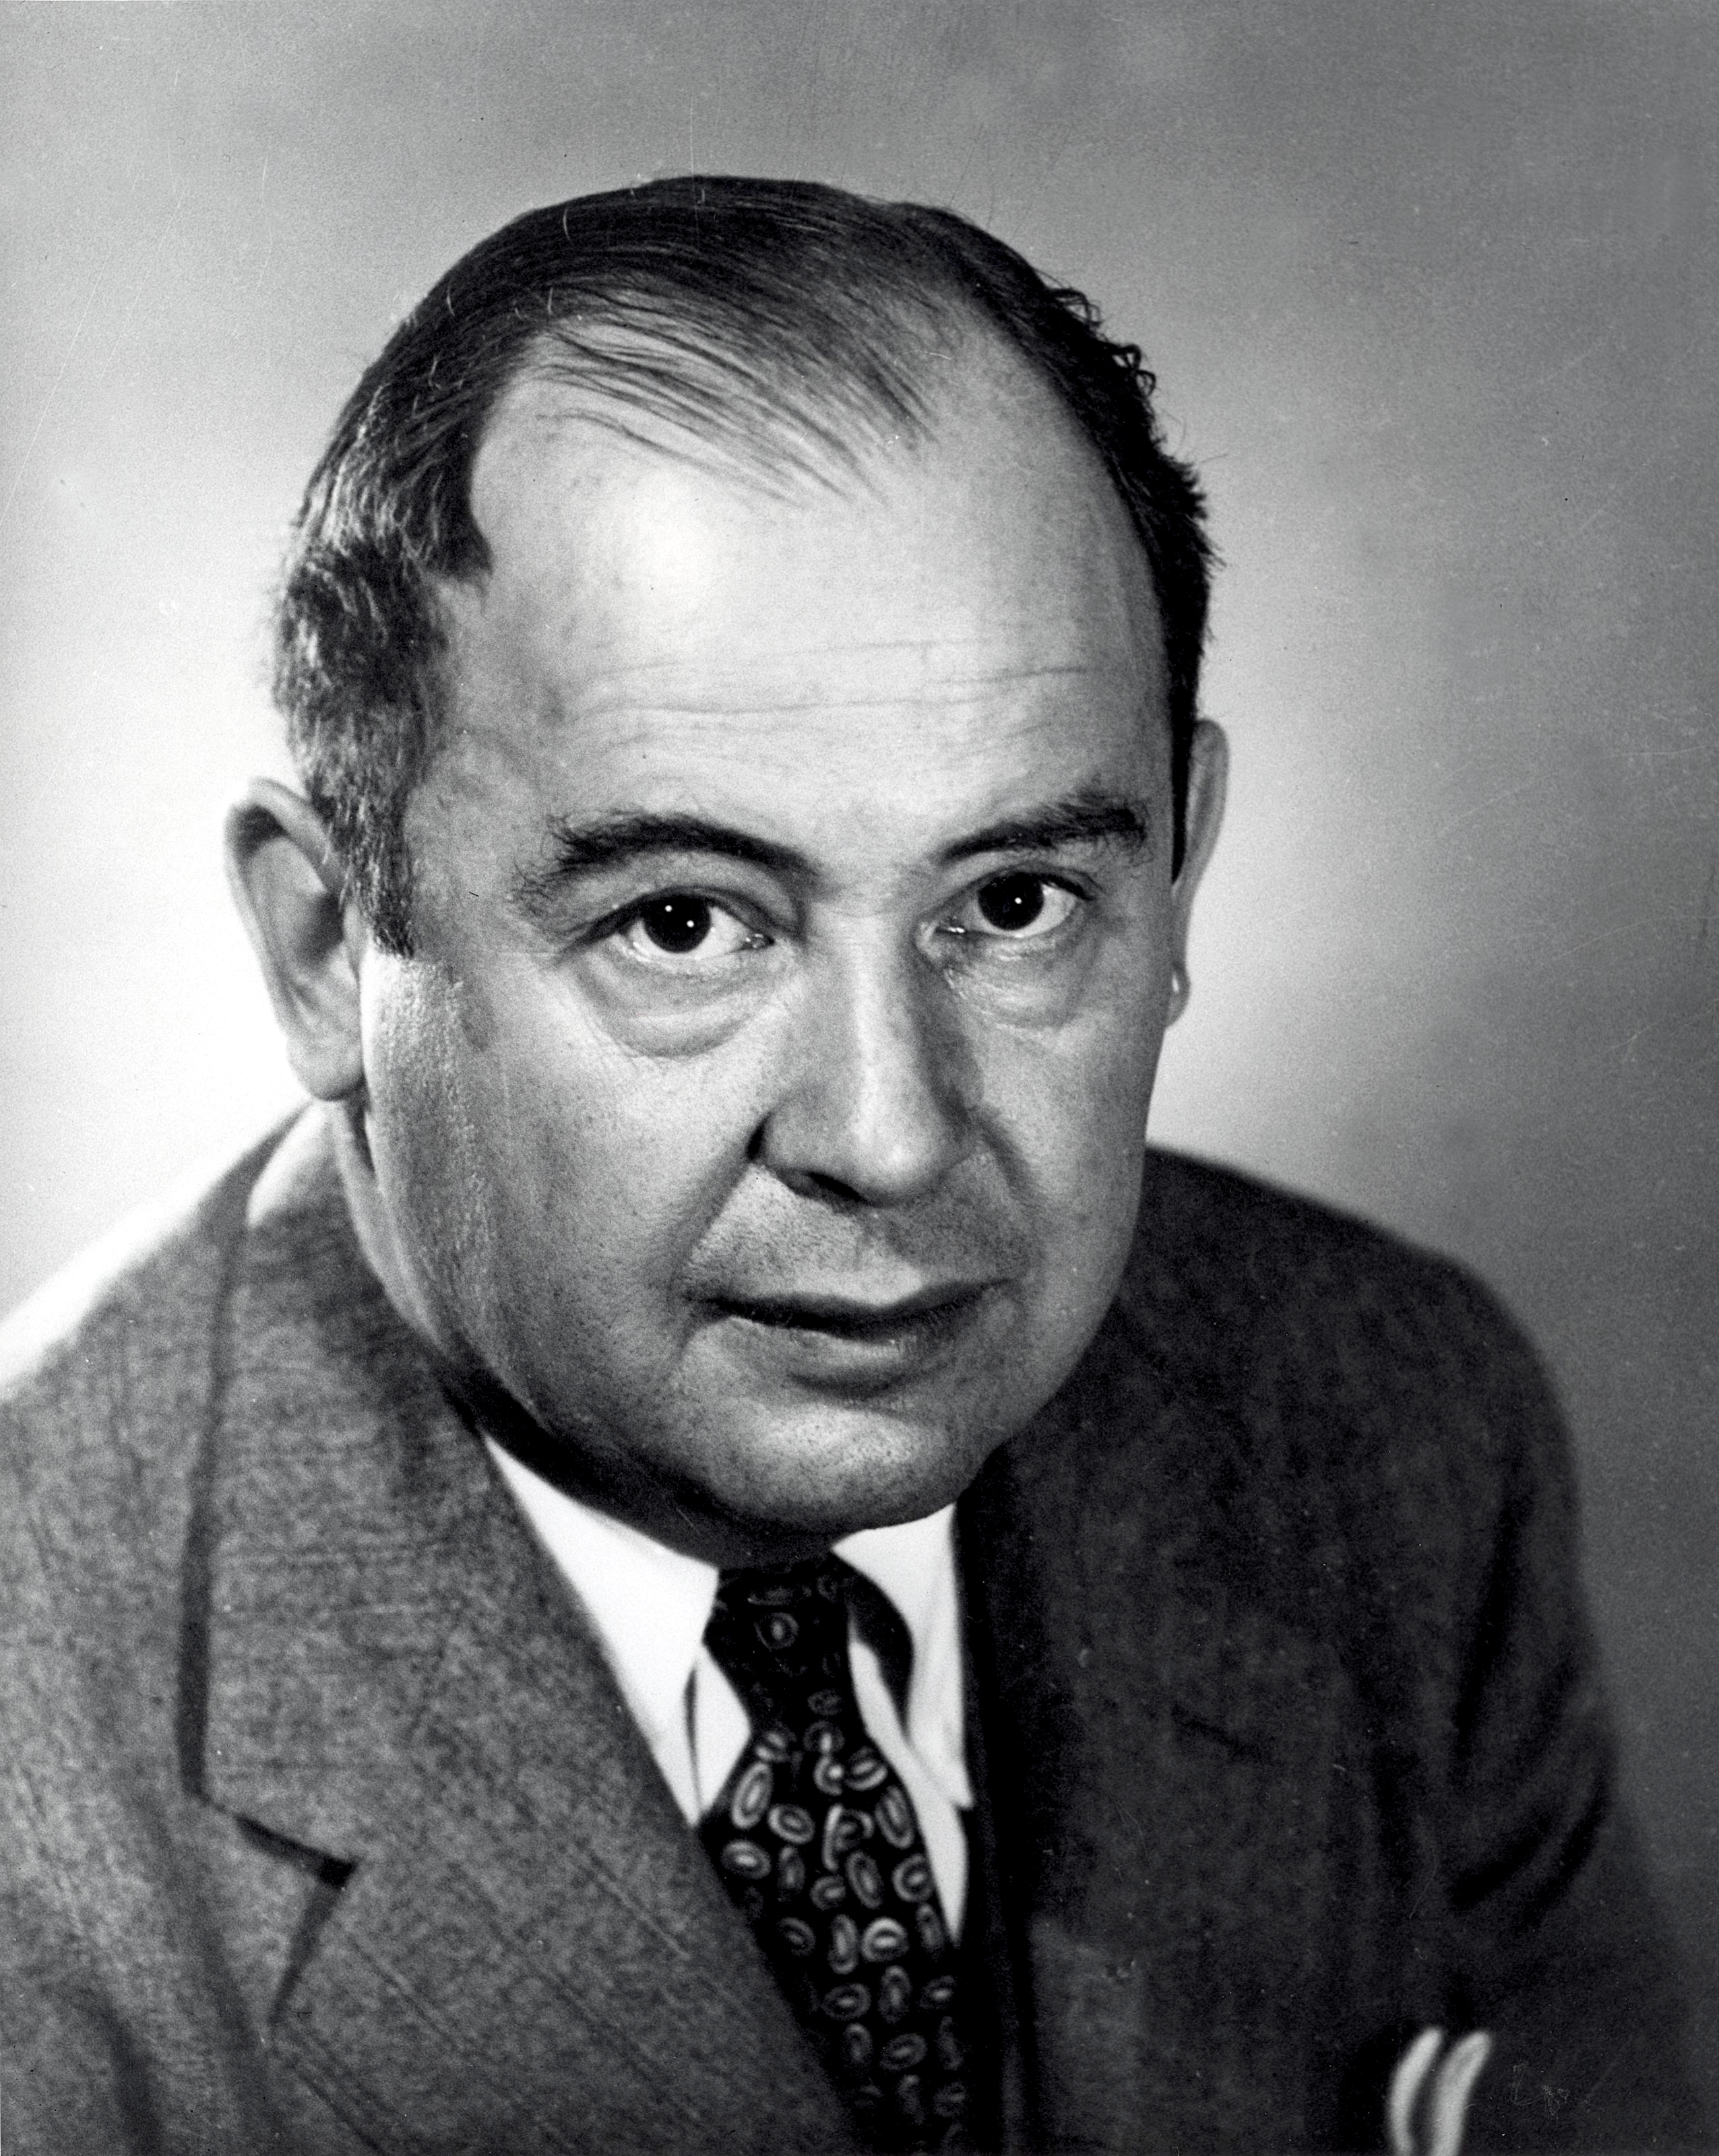
\includegraphics[height=5.5cm, width=4.5cm]{neuman}\\
			Figura: John von Neumann.
		\end{tabular}
		& \begin{tabular}{l}
			\parbox{0.4\linewidth}{%  change the parbox width as appropiate				
				A arquitetura de von Neumann é uma arquitetura de um computador digital que possibilita uma máquina digital armazenar os seus programas no mesmo espaço de memória que os dados, podendo assim manipular tais programas. \\~\\
				
				``Não há sentido em em ser preciso quando não se sabe sobre o que está a falar" - von Neumann. 
			}
		\end{tabular}  \\
	\end{tabular}
\end{frame}


\begin{frame}{Arquitetura de von Neumann}		
A máquina proposta por von Neumann possui as seguintes componentes:
			
\begin{enumerate}
\item Uma \textbf{memória};
\item Uma \textbf{unidade aritmética e lógica};
\item Uma \textbf{unidade central de processamento} (CPU), composto por diversos registradores;
\item Uma \textbf{unidade de controle}, cuja função é a mesma da tabela de controle de uma Máquina de Turing universal (estabelece as mudanças de estado por meio das entradas).
\end{enumerate}
\end{frame}

\begin{frame}{Compilador}
\begin{block}{\textbf{O que é um compilador?}}
\pause\textbf{Resposta}: Um compilador é um programa de computador ou mesmo um grupo de programas que é responsável por traduzir um código fonte escrito em uma linguagem compilada à um programa equivalente do ponto de vista semântico. 
\end{block}
\vspace{0.2cm}
\pause O compilador traduz o código fonte de uma linguagem de programação de médio/alto nível para uma linguagem de programação de baixo nível (a exemplo da linguagem \texttt{Assembly} ou código de máquina).
\end{frame}

\begin{frame}{Compilador}
\begin{block}{\textbf{Bytecode?}}
\pause Alguns compiladores traduzem o código para um formato intermediário, denominado de \textbf{bytecode} que é um código de baixo nível. Sendo assim, o bytecode não é imediatamente um arquivo executável.
\end{block}

\pause \textbf{Observação}: Chamamos de linguagem de baixo nível as linguagem que trabalhando próximo ao hardware. Baixo nível, médio nível ou alto nível em nada em a ver com a qualidade da linguagem de programação.\\~\\

\pause \textbf{Importante}: Jamais confunda bytecode com código de máquina. Bytecode é um formato intermediário que irá ser interpretado em uma máquina virtual que fará a execução. 
\end{frame}

\begin{frame}{Compilador}
A vantagem do bytecode é que o código torna-se mais \textbf{portável}, isto é, podemos com o resultado da compilação executar o código proveniente de um processo de compilação em diversas arquiteturas distintas. Dessa forma, o bytecode irá produzir o mesmo resultado esperado em qualquer arquitetura que possua uma máquina virtual que execute o código intermediário.\\~\\

\textbf{Exemplos de linguagem que converte o código fonte para bytecode}: \texttt{Java} que corre o código sobre a máquina virtual \texttt{Java}, \texttt{.NET} que corre o código sobre a \textit{Common Language Runtime}. 
\end{frame}

\begin{frame}{Compilador}
\begin{block}{\textbf{Código Objeto e Código de Máquina}}
	O \textbf{código de máquina} é um código binário (0 e 1) que poderá ser executado diretamente pela CPU.\\~\\
	
	Se abrirmos um arquivo de código de máquina em um editor de texto, veríamos um emaranhado de caracteres sem sentido. É possível ter acesso ao código de máquina em formato hexadecimal por meio de softwares adequados.\\~\\
	
	O \textbf{código objeto} é a saída de um processo de compilação e trata-se de uma parte do código de máquina que ainda não foi vinculado em um programa completo por meio de um \textbf{linker}.
\end{block}
\end{frame}

\begin{frame}{Abrindo um Código de Maquina}
Ao tentarmos abrir um código de máquina em um editor de texto comum visualizamos algo sem sentido como a sequência de caracteres abaixo:\\~\\
\pause \begin{figure}
\centering
\includegraphics[scale=0.45]{abrindo_maquina}
\end{figure}
Porém, é possível ter acesso ao código de máquina utilizando editores próprios que apresentam o código em hexadecimal, como o exemplo que segue no \textit{frame} seguinte.
\end{frame}

\begin{frame}[fragile]{Compilador}
\begin{verbatim}
	C:\Utility>debug v.exe
	-d 0 100
	0E3D:0000  CD 20 FF 9F 00 9A F0 FE ........O.....
	0E3D:0010  F0 07 17 03 F0 07 DF 07 ................
	0E3D:0020  FF FF FF FF FF FF FF FF ..............L.
	0E3D:0030  D0 0C 14 00 18 00 3D 0E ......=.........
	0E3D:0040  05 00 00 00 00 00 00 00 ................
	0E3D:0050  CD 21 CB 00 00 00 00 00 .!...........
	0E3D:0060  20 20 20 20 20 20 20 20 .....
	0E3D:0070  20 20 20 20 20 20 20 20 ........
	0E3D:0080  00 0D 76 2E 65 78 65 0D ..v.exe.DOWS\sys
	0E3D:0090  74 65 6D 33 32 5C 64 6F tem32\dosx..da r
	0E3D:00A0  65 64 65 20 28 63 61 72 ede (carregar an
	0E3D:00B0  74 65 73 20 64 6F 20 64 tes do dosx.exe)
\end{verbatim}
\end{frame}


\begin{frame}{Compilador}
\begin{figure}
\centering
\includegraphics[scale=0.13]{compilador}
\end{figure}
\hspace{1cm}Figura: Diagrama (funcionamento de uma compilador).
\end{frame}

\begin{frame}{Compilador}	
Alguns autores citam linguagens compiladas em que a tradução do código gera código em \texttt{C}.\vspace{0.5cm}
\begin{block}{\textbf{Maiores detalhes na referência abaixo}}
Cooper, Torczon. Engineering a Compiler (em inglês). San Francisco: Morgan Kaufmann, 2003. p. 2. ISBN 1-55860-698-X.
\end{block}
\end{frame}

\begin{frame}{Compilador}
\begin{block}{\textbf{Importante}}
É importante não confundir \textbf{compilador} com \textbf{tradutor} ou \textbf{filtro} que também pode ser chamado de \textbf{conversor de linguagem}.
\end{block}
\vspace{0.3cm}
O conversor de linguagem é responsável por converter o código de uma linguagem de alto nível para o código de um outra linguagem de médio/alto nível.\\~\\

\textbf{Observação}: Um programa que traduz uma linguagem de programação de baixo nível para uma linguagem de programação de alto nível é denominado de \textbf{descompilador}.
\end{frame}

\begin{frame}{Compilador}
	\begin{tabular}{cl}  
		\begin{tabular}{c}
			\includegraphics[height=5.5cm, width=4.5cm]{Grace_Hopper}\\
			Figura: Grace Hopper.
		\end{tabular}
		& \begin{tabular}{l}
			\parbox{0.5\linewidth}{%  change the parbox width as appropiate				
			O primeiro compilador foi escrito por Grace Hopper no ano de 1952 para a linguagem de programação \texttt{A-0}.\vspace{0.3cm}
			
			Grace Hopper foi analista de sistemas da Marinha dos Estados Unidos. Ela também criou o primeiro compilador para a linguagem \texttt{COBOL}.\vspace{0.3cm}
			
			
			\textbf{Curiosidade}: É atribuído à Grace Hopper o termo \textbf{bug} utilizado para designar uma falha no código fonte. 
			}
		\end{tabular}  \\
	\end{tabular}
\end{frame}

\begin{frame}{Compilador}
	\begin{tabular}{cl}  
		\begin{tabular}{c}
			\includegraphics[height=5.5cm, width=4.5cm]{Grace_Hopper}\\
			Figura: Grace Hopper.
		\end{tabular}
		& \begin{tabular}{l}
			\parbox{0.5\linewidth}{%  change the parbox width as appropiate				
			Grace Hopper é graduada em matemática e física em 1928 e em 1930 concluiu seu mestrado na Yale University. Em 1934, na mesma Universidade, ela obteve o seu PhD em matemática.  
			}
		\end{tabular}  \\
	\end{tabular}
\end{frame}

\begin{frame}{Compilador}
Muitos compiladores incluem um \textbf{pré-processador} que é um programa separado mas invocado pelo compilador antes do início do processo de tradução.\\~\\

Normalmente é pre-processador responsável por mudanças no código fonte destinadas de acordo com decisões tomadas em tempo de compilação.\\~\\

Em programas em \texttt{C} há diversas diretivas para inclusão de novos códigos disponíveis em bibliotecas ou código a parte escrito pelo programador que é informado sua existência por meio de diretivas para o pre-processador.\\~\\ 
\end{frame}

\begin{frame}{Compilador}
\textbf{Exemplo}: É o pré-processador que substitui os comentários do código fonte por espaços em branco. Ou seja, o compilador não ``enxerga" nenhum comentário.\\~\\
\textbf{Exemplos de linguagens compiladas}: \texttt{C}, \texttt{C++}, \texttt{Fortran}, \texttt{Objecte-C}, \texttt{Ocalm}, \texttt{BASIC}, \texttt{COBOL}, \texttt{Ada}, \texttt{D}, entre outras.
\end{frame}

\begin{frame}{Interpretador}
\begin{block}{\textbf{O que é um interpretador?}}
\textbf{Resposta}: Interpretadores são programas de computador que tem a finalidade  de ler o código-fonte de uma linguagem de programação interpretada e o converte em um código executável.
\end{block}
\vspace{0.3cm}
\pause \textbf{Seu funcionamento pode ser, em geral, de duas formas}:
\begin{itemize}
	\item O interpretador lê linha-por-linha e converte o código fonte em código objeto (ou bytecode) a medida que vai executando o programa.
	\pause \item O interpretador converte o código fonte por inteiro e depois o executa.
\end{itemize}
\pause \textbf{Exemplos de linguagens interpretadas}: \texttt{R}, \texttt{Perl}, \texttt{Python}, \texttt{Haskell}, \texttt{Lua}, \texttt{Ruby}, \texttt{Lisp}, \texttt{JavaScript}, entre outras.
\end{frame}

\begin{frame}[fragile]{Programando em \C}
Na linguagem \texttt{C} existe uma função em que são colocadas todas as instruções que queremos que sejam executadas. Essa função chama-se \texttt{main()}, e todo código a executar é colocado entre \texttt{\{\}}.\\~\\

Ao conjunto de código existente dentro de \texttt{\{\}} chamaremos de \textbf{bloco}.\\~\\

\textbf{Exemplo}: Compile e execute seu primeiro programa utilizando a IDE Code::Blocks.
\begin{verbatim}
main()
{
}
\end{verbatim}
\end{frame}

\begin{frame}{Programando em \C}
Como podemos observar, este programa faz uma das coisas que mais gosto na vida: não fazer nada. \smiley\\~\\

\pause Observe com atenção cada linha do programa. A primeira linha é composta pela palavra chave \texttt{main} que delimita o local onde todos os programas em \texttt{C} começam.\\~\\

\pause \textbf{Observação}: Para indicar que \texttt{main} é uma função, tal palavra chave é seguida com parênteses - \texttt{main()} pois \textbf{em \texttt{C} qualquer função tem que ser seguida por parênteses}.
\end{frame}

\begin{frame}{Programando em \C}
\begin{block}{\textbf{Importante}}
Os parênteses sem mais nada após o nome da função indicam que a função não recebe qualquer informação do mundo exterior.
\end{block}
\pause \begin{block}{\textbf{Mais Importante Ainda}}
\texttt{C} é uma linguagem \textbf{Case Sensitive}, isto significa que \texttt{C} faz diferenciação entre maiúscula e minúscula. Assim, não são a mesma coisa escrever \texttt{main()}, \texttt{Main()}, \texttt{MAIN()}, \texttt{mAiN()}, etc.
\end{block}
\pause \textbf{Dica}: Todas as funções em \texttt{C} são escritas em letra minúscula, e só se deve utilizar letras maiúsculas quando desejamos utilizar variáveis, mensagens ou funções escritas por nós.
\end{frame}

\begin{frame}[fragile]{Programando em \C}
No exemplo anterior, o código não executa nada uma vez que não há código dentro do bloco de instruções composto pela função \texttt{main()}.\\~\\

\textbf{Nota}: É possível que o seu compilador tenha apresentado um \textit{WARNING} com uma mensagem semelhante a ``\textbf{Function should return value}"ou ``\textbf{main: no return value}". Isso se deve ao fato de que a principio estamos utilizando um compilador para \texttt{C++}. Duas possíveis soluções caso isso ocorra são:\\~\\
\begin{enumerate}
	\pause \item Ignorar o aviso. \textit{WARNING} não é erro mas devemos prestar atenção nos avisos para evitarmos problemas.
	\pause \item Coloque a palavra chave \texttt{void} antes da função \texttt{main()} na forma que segue.
\end{enumerate}
\end{frame}

\begin{frame}[fragile]{Programando em \C}
\begin{verbatim}
void main()
{
}
\end{verbatim}
\pause Mais tarde nós saberemos o porquê do uso de \texttt{void}.\\~\\

\pause Vamos agora escrever um novo programa que faz algo mais interessante do que nada. Considere o exemplo que segue: 
\end{frame}

\begin{frame}[fragile]{Programando em \C}
\textbf{Exemplo}: 
\begin{verbatim}
1: #include <stdio.h>
2: main()
3: {
4:      printf("Hello Mundo Cruel");
5: }
\end{verbatim}
\pause Esse código é em tudo semelhante ao anterior, com a exceção da existência de uma linha de código entre as chaves.\\~\\

\pause A linha 4 é responsável pela apresentação da mensagem que desejamos imprimir: ``Hello Mundo Cruel".
\end{frame}

\begin{frame}{Programando em \C}
\begin{block}{\textbf{Importante}}
Sempre que queremos tratar conjunto de caracteres temos que colocá-los entre aspas, para que sejam considerados como um todo, isto é, devemos fazer \texttt{"Hello Mundo Cruel"} para o exemplo acima.
\end{block}
\pause \begin{block}{\textbf{A função \texttt{printf()}}}
Uma das funções que permite a escrita na tela é a função \texttt{printf()} = \textbf{print} $+$ \textbf{f}ormatado. Como trata-se de uma função, há a necessidade de colocar os parênteses.	
\end{block}
\pause Dentro do parênteses é feita a comunicação com a função. Nesse exemplo, passamos a \textbf{\textit{string}} (cadeia de caracteres) que queremos que seja escrita - \texttt{printf("Hello Mundo Cruel")}.
\end{frame} 

\begin{frame}{Programando em \C}
\begin{block}{\textbf{Muito Importante}}
\begin{enumerate}
	\pause \item Em \texttt{C}, cada instrução deve ser terminada com um ponto-e-vírgula (;), obtendo-se assim a linha 4 do programa - \texttt{printf("Hello Mundo Cruel");}
	\pause \item Preste muita atenção e perceba que o caractere \texttt{"} (aspas) é um \textbf{único} caractere e não pode ser substituído pelo caractere aspas simples \texttt{'} nem muito menos por duas aspas simples \texttt{''}.
\end{enumerate}
\end{block}
\pause\textbf{Observação}: A linguagem \texttt{C} não possui mecanismos de \textbf{Entrada/Saída} (\textbf{Input/Output}). Dessa forma, precisamos recorrer a um conjunto de funções em \textbf{bibliotecas de funções} (\textbf{bibliotecas}).
\end{frame}

\begin{frame}{Programando em \C}
Dessa forma, precisamos adicionar à linguagem \texttt{C} um conjunto de funções que, ``por defeito", ela não nos proporciona.\\~\\

\pause Para ter acesso a esse conjunto de funções teremos que incluir a sua definição no nosso código fonte.\\~\\

\pause No exemplo anterior fazemos isso com a linha \texttt{\#include <stdio.h>}.
\end{frame}

\begin{frame}{Programando em \C}
\pause \begin{block}{\textbf{A linha \texttt{\#include <stdio.h>} é \C?}}
\textbf{Resposta}: A linha \texttt{\#include <stdio.h>} \textbf{não} é \texttt{C} mas uma diretiva que indica ao pré-processador que deverá ser adicionado antes da compilação um arquivo existente em alguma parte no disco do computador. Tal arquivo nesse caso é \textbf{stdio.h}.
\end{block}
\vspace{0.3cm}
\pause Esses arquivos são normalmente chamados de arquivos cabeçalhos e tem extensão \texttt{.h}, pois não têm código, mas apenas os cabeçalhos (\textit{\textbf{h}eaders}) das funções que apresentam. Normalmente são chamados de \textit{\textbf{header files}}.\\~\\

\pause \texttt{\#include <stdio.h>} $=$ adiciona o arquivo \textbf{stdio.h} ao meu programa \textbf{exatamente nesta posição}.
\end{frame}

\begin{frame}{Programando em \C}
\begin{block}{\textbf{Por que não colocamos \texttt{;} (ponto-e-vírgula) depois de \texttt{\#include <stdio.h>}}?}
\textbf{Resposta}: Porque, como foi mencionado anteriormente, \texttt{\#include <stdio.h>} é uma diretiva do pré-processador. Dessa forma, \texttt{\#include <stdio.h>} não é um comando de \C.
\end{block}
\vspace{0.3cm}
\textbf{Nota}: Não colocamos \texttt{;} (ponto-e-vírgula) ao final de instruções que não são de \C.\\~\\

O arquivo \texttt{stdio.h} permite o acesso a todas as funções de Entrada/Saída que necessitamos, em que \textbf{stdio} significa \textbf{standard input/output}.
\end{frame}

\begin{frame}[fragile]{Programando em \C}
O programa que imprime na tela a mensagem "Hello Mundo Cruel" poderia ser programado de uma forma diferente e equivalente da forma que segue.\\~\\

\textbf{Exemplo}: Dividindo a mensagem em mais de um \texttt{printf}.

\begin{verbatim}
1: #include <stdio.h>
2: main()
3: {
4:     printf("Hello");
5:     printf(" ");
6:     printf("Mundo");
7:     printf(" ");
8:     printf("Cruel");
9: }
\end{verbatim}
\end{frame}

\begin{frame}[fragile]{Programando em \C}
O compilador de \texttt{C} é, em geral, liberal no que diz respeito à forma como escrevemos (\textbf{identamos}) o código. Este pode ser escrito de modo que cada programador possa entender.\\~\\

\pause \textbf{Exemplo}: Compile o código \texttt{C} que segue abaixo.

\begin{verbatim}
#include <stdio.h>
main        (  )  {
   printf(
"Hello"
);
   printf(   "Mundo "           )
;   printf(         "Cruel"                  );}
\end{verbatim}
\end{frame}

\begin{frame}{Programando em \C}
\textbf{Observação}: Espaços em branco são ignorados pelo compilador de \C.\\~\\

Nos programas que escrevem a frase ``Hello Mundo Cruel" apresentados anteriormente observa-se que o cursor fica posicionado imediatamente após a palavra ``Cruel". Isso ocorre pelo fato de o programador não ter mandado o cursor mudar de linha após a escrita da mensagem.\\~\\

Normalmente as linguagens de programação apresentam funções ou instruções distintas para realizar uma escrita na tela seguida ou não de uma nova linha. Em \texttt{C} a filosofia é outra.\\~\\
\end{frame}

\begin{frame}[fragile]{Programando em \C}
\begin{block}{\textbf{Como podemos mudar de linha ao escrever uma mensagem?}}
	\textbf{Resposta}: Tradicionalmente a mudança de linha é denominada \textbf{New Line}, e em \texttt{C} é representada pelo símbolo \texttt{\barra n}.
\end{block}

\textbf{Exemplo}: Considere o exemplo que segue.
\begin{verbatim}
1: #include <stdio.h>
2: void main()
3: {
4:     printf("Hello Mundo Cruel\n");
5: }
\end{verbatim}
\end{frame} 

\begin{frame}[fragile]{Programando em \C}
\textbf{Observação}: O caractere especial \textit{New Line} representado por \texttt{\barra n} é um caractere como qualquer outro. Assim, poderemos utilizar \texttt{\barra n} quantas vezes acharmos necessário. Nesse caso, poderíamos fazer:\\~\\

\textbf{Exemplo}: Considere o exemplo que segue:

\begin{verbatim}
1: #include <stdio.h>
2: void main()
3: {
4: 	printf("Hello\n\n Mundo\nCruel);
5: }
\end{verbatim}
\end{frame}

\begin{frame}[fragile]{Programando em \C}
\textbf{Exercício}: Escreva um programa em \texttt{C} que possui a seguinte saída:

\begin{verbatim}
C
eh uma otima linguagem. Eu serei
um grande programador em
C!
\end{verbatim}
\pause \textbf{Uma solução}: 
\begin{verbatim}
1: #include <stdio.h>
2: void main()
3: {
4:     printf("C\n");
5:     printf("eh uma otima linguagem. Eu serei");
6:     printf("um grande programado em");
7:     printf("C!");
8: }
\end{verbatim}
\end{frame}

\begin{frame}[fragile]{Programando em \C}
	\textbf{Exercício}:
	\pause \textbf{Outra solução utilizando apenas um \texttt{printf()}}
	\begin{verbatim}
	#include <stdio.h>
	void main()
	{
	    printf("C\neh uma otima linguagem.
	    Eu seirei\num grande programador em\nC!");
	}
	\end{verbatim}
\end{frame}

\begin{frame}[fragile]{Programando em \C}
Suponha agora que queremos escrever a seguinte mensagem na tela do computador.\\~\\

\pause \textbf{Hoje eh um dia "LINDO" com uma aula linda!!!}\\~\\

\pause \textbf{Exemplo (com erro de compilação)}: Muitos seriam tentados a pensar no programa que segue.
\begin{verbatim}
1: #include <stdio.h>
2: main()
3: {
4:     printf("Hoje eh um dia "LINDO" com uma aula
5:             linda!!!");
6: }
\end{verbatim}
\end{frame}

\begin{frame}{Programando em \C}
\begin{block}{\textbf{Por que do erro do código acima?}}
\textbf{Resposta}: O erro ocorre porque até a primeira ocorrência do símbolo \texttt{"} a linguagem \texttt{C} entende que estamos escrevendo \texttt{"Hoje eh um dia "}. Porém existe algo a mais dentro da função \texttt{printf()} que não é (\textit{string}). 
\end{block}
\vspace{0.5cm}
\textbf{Nota}: Chamamos de \textbf{string} uma cadeia de caracteres. Strings em \texttt{C} é definida entre aspas dupla (ex. \texttt{"minha string"}).
\end{frame}

\begin{frame}{Programando em \C}
\begin{figure}
	\centering
	\includegraphics[scale=0.4]{homer}
\end{figure}

\begin{block}{\textbf{Se as aspas servem para delimitar uma string, como poderemos escrever uma frase (string) em que as aspas sejam um caractere não delimitador?}}
\pause \textbf{Resposta}: Coloque \texttt{\barra} antes das aspas que se pretende escrever na \textit{string}. Assim, as aspas serão tratadas como caracteres normais.
\end{block}
\end{frame}

\begin{frame}[fragile]{Programando em \C}
\textbf{Exemplo}: Para que possamos escrever a frase corretamente na tela do computador, considere o programa abaixo.

\begin{verbatim}
1: #include <stdio.h>
2: void main()
3: {
4:     printf("Hoje eh um dia \"LINDO\" com uma aula
5:             linda!!!");
6: }
\end{verbatim}
\end{frame}

\begin{frame}{Programando em \C}
\begin{table}[]
	\centering
	\caption{O caractere especial \barra.}
	\label{my-label}
	\begin{tabular}{l|l}
		\hline
		\barra 7     & \textit{Bell} (sinal sonoro do computador) \\
		\barra a     & \textit{Bell} (sinal sonoro do computador  \\
		\barra b     & \textit{BackSpace}                         \\
		\barra n     & \textit{New Line} (mudança de linha)       \\
		\barra r     & \textit{Carroage Return}                   \\
		\barra t     & Tabulação Horizontal                         \\
		\barra v     & Tabulação Vertical                           \\
		\barra\barra & Caractere \barra                             \\
		\barra '     & Caractere aspas simples '                    \\
		\barra "     & Caractere aspas dupla "                      \\
		\barra ?     & Caractere ? (ponto de interrogação)          \\
		\%\%         & Caractere \%      \\
		\hline                           
	\end{tabular}
\end{table}
\end{frame}

\begin{frame}{Programando em \C}
\textbf{Exercício}: Crie alguns programas em \texttt{C} que faz uso de alguns caracteres especiais.\\~\\

É muito importante a prática de se comentar muito bem um código em que escrevemos. Nunca se sabe quando teremos a necessidade de reprogramar o código.\\~\\

É comum em um código não comentado esquecermos o que foi feito em um código fonte programado a muito tempo. \\~\\

\textbf{Observação}: O bom programador segue ``sempre" boas práticas de programação. Comentar bem um código por mais simples que ele seja é uma boa prática de programação.
\end{frame}

\begin{frame}[fragile]{Programando em \C}
\begin{block}{\textbf{Como são feitos comentários em \C?}}
\textbf{Resposta}: Comentários em \texttt{C} são colocados entre \texttt{/* */} (\texttt{/* AQUI É UM COMENTÁRIO */}).\\~\\
\end{block}
\textbf{Alguns exemplos de cabeçalhos de programas escritos em \texttt{C} são}:

\begin{verbatim}
/* programa.c: Empresa Comentários e CIA */
/* AUTOR: Pedro Rafael                   */
/* DATA: 02/02/2017                      */
\end{verbatim}
Acima temos três comentários em que cada um deles estão entre \texttt{/* */}. Porém, poderíamos ter feito:
\end{frame}

\begin{frame}[fragile]{Programando em \C}
\begin{verbatim}
/* programa.c: Empresa Comentários e CIA
 * AUTOR: Pedro Rafael                   
 * DATA: 02/02/2017                      
*/
\end{verbatim}
ou então:
\begin{verbatim}
/******************************************
 * programa.c: Empresa Comentários e CIA  *
 * AUTOR: Pedro Rafael                    *
 * DATA: 02/02/2017                       *
 ******************************************/
\end{verbatim}
\textbf{Observação}: Os asteriscos horizontais ou verticais \textbf{não} tem nenhum significado especial. Eles apenas fazem parte do que queremos comentar.
\end{frame}

\begin{frame}{Programando em \C}
\begin{block}{\textbf{Importante}}
Os comentários podem também serem colocados dentro de expressões ou instruções. 
\end{block}
\vspace{0.3cm}
\textbf{Exemplo}: Poderíamos fazer:\\~\\ \texttt{printf("Bom dia querido professor, nós o adoramos!" /* É mentira :P */); /* Notar o ponto-ponto e vírgula */}\\~\\

\textbf{Dica}: Particularmente, não acho uma boa prática de programação comentar no interior de instruções ou expressões. Tal postura tornará o código difícil de ser entendido.
\end{frame}
 
\begin{frame}[fragile]{Programando em \C}
\begin{block}{\textbf{Importante}}
Os compiladores de \texttt{C} \textbf{não} permitem, em geral, comentários dentro de comentários.
\end{block}
\textbf{Exemplo}: Comentários dentro de comentários não são permitidos, em geral, em \C.
\begin{verbatim}
/* Meu primeiro comentário.
/* Meu segundo comentário sobre or primeiro
   comentário. */
*/
\end{verbatim}
\textbf{Nota}: Alguns compiladores permitem o uso de comentários dentro de comentários. Porém, tão opção não é reconhecida pelo ANSI. 
\end{frame} 
 


\end{document}